\documentclass[a4paper,12pt]{article}
\usepackage{amsmath}
\usepackage{pdfpages}
\usepackage[utf8]{inputenc}
\usepackage{hyperref}
\usepackage{listings}
\usepackage{xcolor}
\usepackage{fancyhdr}
\definecolor{codegreen}{rgb}{0,0.6,0}
\definecolor{codegray}{rgb}{0.5,0.5,0.5}
\definecolor{backcolour}{rgb}{0.95,0.95,0.92}
\definecolor{linkcolor}{HTML}{799BF3}
\definecolor{urlcolor}{HTML}{799BF3} 
\hypersetup{pdfstartview=FitH,  linkcolor=linkcolor,urlcolor=urlcolor, colorlinks=true}


\lstdefinestyle{mystyle}{
    backgroundcolor=\color{backcolour},   
    commentstyle=\color{codegreen},
    keywordstyle=\color{blue},
    numberstyle=\tiny\color{codegray},
    basicstyle=\ttfamily\footnotesize,
    breakatwhitespace=false,         
    breaklines=true,                 
    captionpos=b,                    
    keepspaces=true,                 
    numbers=left,                    
    numbersep=5pt,                  
    showspaces=false,                
    showstringspaces=false,
    showtabs=false,                  
    tabsize=2
}

\lstset{style=mystyle}

\pagestyle{fancy}
\fancyhf{}
\lhead{Contol theory Homework \#4 report}
\rhead{Anton Brisilin, BS18-02 Student}
\fancyfoot[R]{\today}
\fancyfoot[C]{\thepage}
\renewcommand{\footrulewidth}{1pt}
\renewcommand{\headrulewidth}{1pt}

\begin{document}
\section{Task 1}
My name is \textit{Anton Brisilin}, and my email is 
\textit{a.brisilin@innopolis.university}, so my generated variant is \textbf{F}.
\section{Task 2}
    \subsection{Write equations of motion of the system in manipulator form}
    Source system of equations:
    \begin{equation}\label{source_eq}
        \begin{cases}
            (M+m)\ddot{x}-mlcos(\theta)\ddot{\theta}+mlsin(\theta)\dot\theta^2=F\\
            -cos(\theta)\ddot{x}+l\ddot{\theta}-gsin(\theta)=0
        \end{cases}
    \end{equation}
    Manipulator form:
    \begin{equation}
        \begin{cases}\label{desired_form}
            M(q)\ddot{q}+n(q,\dot{q})=Bu\\
            u=F\\
            q=\begin{bmatrix}x \\ \theta\end{bmatrix}
        \end{cases}
    \end{equation}
    My goal is to transform (\ref{source_eq}) to the form of (\ref{desired_form}). 
    To do it I can transform first equation of (\ref{source_eq}) to the form of
    \begin{equation}\label{first_part}
        \begin{bmatrix}
            M+m & -mlcos(\theta)
        \end{bmatrix}
        \begin{bmatrix}
            \ddot x \\ 
            \ddot\theta
        \end{bmatrix}
         + (mlsin(\theta)\dot\theta^2) = [1]u
    \end{equation}
    This already is motion equation in standart (manipulator) form. But for this
    equation to describe motion of our system it should also consider second
    equation of system (\ref{source_eq}). Therefore, our equation (\ref{first_part})
    becomes
    \begin{equation}
        \begin{bmatrix}
            M+m & -mlcos(\theta) \\
            -cos(\theta) & l
        \end{bmatrix}
        \begin{bmatrix}
            \ddot x \\ 
            \ddot\theta
        \end{bmatrix}
        +
        \begin{bmatrix}
            mlsin(\theta)\dot\theta^2\\
            -gsin\theta
        \end{bmatrix}
        = 
        \begin{bmatrix}
            1\\
            0
        \end{bmatrix}u
    \end{equation}
    And with substitution of numbers from variant \textbf{F}:
    \begin{equation}
        \begin{bmatrix}
            11.6 & -7.298 * cos(\theta) \\
            -cos(\theta) & 0.89
        \end{bmatrix}
        \begin{bmatrix}
            \ddot x \\ 
            \ddot\theta
        \end{bmatrix}
        +
        \begin{bmatrix}
            7.298*sin(\theta)\dot\theta^2\\
            -9.81*sin\theta
        \end{bmatrix}
        = 
        \begin{bmatrix}
            1\\
            0
        \end{bmatrix}u
    \end{equation}
    \subsection{Write dynamics of the system in control affine nonlinear form}
    Control affine nonlinear form:
    \begin{equation}\label{desired_form2}
        \begin{cases}
            \dot z = f(z) + g(z)u\\
            u=F\\
            z = 
            \begin{bmatrix}
                x&
                \theta&
                \dot x&
                \dot \theta    
            \end{bmatrix}^T
        \end{cases}
    \end{equation}
    It's pretty obvious that one can easily express $\dot x$ and $\dot \theta$ 
    through $z$:
    \begin{equation}
        \begin{bmatrix}
            \dot x\\
            \dot \theta
        \end{bmatrix}
        =
        \begin{bmatrix}
            \dot x\\
            \dot \theta    
        \end{bmatrix}
        +
        \begin{bmatrix}
            0\\
            0\\    
        \end{bmatrix}F
    \end{equation}
    So the goal is to express $\ddot x$ and $\ddot \theta$ through $x, \dot x, 
    \theta$ and $\dot \theta$. From the second equation of system (\ref{source_eq}):
    \begin{equation}\label{x_ddot}
        \ddot x = \frac{l\ddot\theta - gsin(\theta)}{cos(\theta)}
    \end{equation}
    Substituting (\ref{x_ddot}) to the first equation of (\ref{source_eq}), we can 
    express $\ddot{\theta}$:
    \begin{gather*}
        \ddot{\theta}=
        \frac
        {(M+m)\ddot{x}+mlsin(\theta)\dot \theta^2-F}
        {mlcos(\theta)}
        \\
        \ddot{\theta}=
        \frac
        {(M+m) (l\ddot \theta - gsin(\theta))}
        {mlcos^2(\theta)}
        +
        tg(\theta) \dot \theta^2
        - 
        \frac
        {F}
        {mlcos(\theta)}
        \\
        \ddot{\theta}=
        \frac
        {(M+m)l\ddot\theta}
        {mlcos^2(\theta)}
        - 
        \frac
        {(M+m)gsin(\theta)}
        {mlcos^2(\theta)}
        +
        tg(\theta) \dot \theta^2
        - 
        \frac
        {F}
        {mlcos(\theta)}
        \\
        \ddot{\theta}
        \left(
            \frac
            {mlcos^2(\theta)-(M+m)l}
            {mlcos^2(\theta)}
        \right)=
        - 
        \frac
        {(M+m)gsin(\theta)}
        {mlcos^2(\theta)}
        +
        tg(\theta)\dot \theta^2 
        -
        \frac
        {F}
        {mlcos(\theta)}
        \\
        \ddot\theta =
        \frac
        {-  \frac
            {(M+m)gsin(\theta)}
            {mlcos^2(\theta)}
            +
            tg(\theta)\dot \theta^2
            - 
            \frac
            {F}
            {mlcos(\theta)}
        }
        {
            \frac
            {mlcos^2(\theta)-(M+m)l}
            {mlcos^2(\theta)}
        }
        \\
        \ddot\theta = 
        \frac
        {-(M+m)gsin(\theta) + mlcos(\theta)sin(\theta)\dot\theta^2 - Fcos(\theta)}
        {mlcos^2(\theta)-(M+m)l}
        \\
    \end{gather*}
    \begin{equation}\label{theta_ddot}
        \ddot\theta = 
        \frac
        {(M+m)gsin(\theta) - mlcos(\theta)sin(\theta)\dot \theta^2}
        {l((M+m) - mcos^2(\theta))}
        +
        \frac
        {Fcos(\theta)}
        {l((M+m) - mcos^2(\theta))}
    \end{equation}
    Now, substituting (\ref{theta_ddot}) to (\ref{x_ddot}):
    \begin{gather*}
        \ddot x = 
        \frac
        {(M+m)gtg(\theta) - mlsin(\theta)\dot \theta^2}
        {(M+m) - mcos^2(\theta)}
        +
        \frac
        {F}
        {(M+m) - mcos^2(\theta)}
        -
        gtg(\theta)
    \end{gather*}
    \begin{equation}
        \ddot x = 
        \frac
        {- mlsin(\theta)\dot \theta^2 + mgsin(\theta)cos(\theta)}
        {(M+m) - mcos^2(\theta)}
        +
        \frac
        {F}
        {(M+m) - mcos^2(\theta)}
    \end{equation}
    Hence, our system (\ref{source_eq}) in control affine nonlinear form can be
    written as:
    \begin{equation}
        \begin{bmatrix}
            \dot x\\
            \dot \theta\\
            \ddot x\\
            \ddot \theta    
        \end{bmatrix}
        =
        \begin{bmatrix}
            \dot x\\
            \dot \theta\\
            \frac
            {- mlsin(\theta)\dot \theta^2 + mgsin(\theta)cos(\theta)}
            {(M+m) - mcos^2(\theta)}\\
            \frac
            {(M+m)gsin(\theta) - mlcos(\theta)sin(\theta)\dot \theta^2}
            {l((M+m) - mcos^2(\theta))}
        \end{bmatrix}
        +
        \begin{bmatrix}
            0\\0\\
            \frac
            {1}
            {(M+m) - mcos^2(\theta)}\\
            \frac
            {cos(\theta)}
            {(M+m) - mcos^2(\theta)}
        \end{bmatrix}
        u
    \end{equation}
    And with substitution of numbers from variant \textbf{F}:
    % Everything becomes even more ugly
    \begin{equation}
        \begin{bmatrix}
            \dot x\\
            \dot \theta\\
            \ddot x\\
            \ddot \theta    
        \end{bmatrix}
        =
        \begin{bmatrix}
            \dot x\\
            \dot \theta\\
            \frac
            {- 7.298sin(\theta)\dot \theta^2 + 80.442sin(\theta)cos(\theta)}
            {11.6 - 8.2cos^2(\theta)}\\
            \frac
            {113.796sin(\theta) - 7.298cos(\theta)sin(\theta)\dot \theta^2}
            {10.324 - 7.298cos^2(\theta)}
        \end{bmatrix}
        +
        \begin{bmatrix}
            0\\0\\
            \frac{1}
            {11.6 - 8.2cos^2(\theta)}\\
            \frac{cos(\theta)}
            {11.6 - 8.2cos^2(\theta)}\\
        \end{bmatrix}
        u
    \end{equation}
    \subsection{Linearize nonlinear dynamics of the systems around equilibrium point
    $\vec{z} = [0\ 0\ 0\ 0]^T$}
    General form of linearized equation:
    \begin{equation}
        \delta \dot z = A \delta z + B \delta u 
    \end{equation}
    Let's begin with checking, whether $\vec{z} = [0\ 0\ 0\ 0]^T$ is really an 
    equilibrium point:
    \begin{equation}
        \begin{cases}
            \dot x = 0\\
            \dot \theta = 0\\
            \ddot x = 0 +  
            \frac{1}
            {11.6 - 8.2cos^2(\theta)}
            u_e = 0\\
            \ddot \theta = 0 +  
            \frac{cos(\theta)}
            {11.6 - 8.2cos^2(\theta)}u_e =0
        \end{cases}
    \end{equation}
    It's seen that last two equations are true, iff $u_e=0$.
    If our system is in form
    \begin{equation}
        \begin{bmatrix}
            \dot x_1\\
            \dot x_2\\
            \dot x_3\\
            \dot x_4\\
        \end{bmatrix}
        =
        \begin{bmatrix}
            f_1(z,u)\\
            f_2(z,u)\\
            f_3(z,u)\\
            f_4(z,u)\\
        \end{bmatrix}
    \end{equation}
    Then, to linearize it, we should found such matrices $A$ and $B$, that
    \begin{equation}
        \begin{cases}
            A=
            \begin{bmatrix}
                \frac
                {\partial f_1}
                {\partial z_1}|_{z_0,u_0} &
                \frac
                {\partial f_1}
                {\partial z_2}|_{z_0,u_0} &
                \frac
                {\partial f_1}
                {\partial z_3}|_{z_0,u_0} &
                \frac
                {\partial f_1}
                {\partial z_4}|_{z_0,u_0} \\
                \frac
                {\partial f_2}
                {\partial z_1}|_{z_0,u_0} &
                \frac
                {\partial f_2}
                {\partial z_2}|_{z_0,u_0} &
                \frac
                {\partial f_2}
                {\partial z_3}|_{z_0,u_0} &
                \frac
                {\partial f_2}
                {\partial z_4}|_{z_0,u_0} \\
                \frac
                {\partial f_3}
                {\partial z_1}|_{z_0,u_0} &
                \frac
                {\partial f_3}
                {\partial z_2}|_{z_0,u_0} &
                \frac
                {\partial f_3}
                {\partial z_3}|_{z_0,u_0} &
                \frac
                {\partial f_3}
                {\partial z_4}|_{z_0,u_0} \\
                \frac
                {\partial f_4}
                {\partial z_1}|_{z_0,u_0} &
                \frac
                {\partial f_4}
                {\partial z_2}|_{z_0,u_0} &
                \frac
                {\partial f_4}
                {\partial z_3}|_{z_0,u_0} &
                \frac
                {\partial f_4}
                {\partial z_4}|_{z_0,u_0} \\
            \end{bmatrix}\\
            B=
            \begin{bmatrix}
                \frac
                {\partial f_1}
                {\partial u}|_{z_0,u_0} \\
                \frac
                {\partial f_2}
                {\partial u}|_{z_0,u_0} \\
                \frac
                {\partial f_3}
                {\partial u}|_{z_0,u_0} \\
                \frac
                {\partial f_4}
                {\partial u}|_{z_0,u_0} \\
            \end{bmatrix}
        \end{cases}
    \end{equation}
    In our case, functions $f_1, ... f_4$ can be taken from previous part of the
    task. Now let's compute the matrices, considering
    \begin{equation}
        \begin{cases}
        z = 
        \begin{bmatrix}
            z_1\\
            z_2\\
            z_3\\
            z_4\\
        \end{bmatrix} = 
        \begin{bmatrix}
            x\\
            \theta\\
            \dot x\\
            \dot \theta    
        \end{bmatrix}\\
        f_1 = z_3\\
        f_2 = z_4\\
        f_3 = \frac
        {- 7.298sin(z_2)z_4^2 + 80.442sin(z_2)cos(z_2)}
        {11.6 - 8.2cos^2(z_2)}
        +
        \frac{u}
        {11.6 - 8.2cos^2(z_2)}
        \\
        f_4 = \frac
        {113.796sin(z_2) - 7.298cos(z_2)sin(z_2)z_4^2}
        {10.324 - 7.298cos^2(z_2)}
        +
        \frac{cos(z_2)u}
        {11.6 - 8.2cos^2(z_2)}\\
        \end{cases}
    \end{equation}
    And let's select one output among all state variables - I have chosen position
    ($x$). Here is obtained state-space model:\\
    \begin{equation}\label{linearized}
        \begin{cases}
            A=
            \begin{bmatrix}
                0 & 0 & 1 & 0 \\
                0 & 0 & 0 & 1 \\
                0 & 23.66 & 0 & 0\\
                0 & 37.6  & 0 & 0\\
            \end{bmatrix}
            B=
            \begin{bmatrix}
                0 \\
                0 \\
                0.294 \\
                0.294 \\
            \end{bmatrix}\\
            \\
            C=
            \begin{bmatrix}
                1 & 0 & 0 & 0\\
            \end{bmatrix}\ 
            D=
            \begin{bmatrix}
                0
            \end{bmatrix}
        \end{cases}
    \end{equation}
    All the derivatives were computed with Matlab.
    Scripts for differentiation can be found in \texttt{Task2/diff.m}
    \subsection{Stability checking}\label{eigenvals}
    I will check stability with looking to eigenvalues of $A$, obtained in 
    (\ref{linearized}). If all of them have negative real parts, then system is 
    stable. Using \texttt{eig()} from \texttt{numpy} I obtained:
    \begin{equation*}
        eigenvalues = 
        \begin{bmatrix}
            0\\
            0\\
            6.13\\
            -6.13
        \end{bmatrix}
    \end{equation*}
    It can be seen, that there is a positive-valued eigenvalue of $A$, so the 
    linearized system is not stable.
    \subsection{Controllability checking}
    For the linear system to be controllable, the next condition should hold:\\
    If $\dot x = Ax + B$, then rank of $\Gamma = 
    \begin{bmatrix}
        B & AB & A^2B & A^3B
    \end{bmatrix}$ should be equal to the dimension of $A$ (in my case 4).
    Calculation of matrix $\Gamma$ can be found in \texttt{Task2/contr.m}.
    \begin{equation}
        \Gamma = 
        \begin{bmatrix}
        0 & 0.2940 & 0 & 6.9560\\
        0 & 0.2940 & 0 & 11.0544\\
        0.2940 & 0 & 6.9560 & 0\\
        0.2940 & 0 & 11.0544 & 0\\
        \end{bmatrix}
    \end{equation}
    It is visible, that rank of this matrix is 4, which is also confirmed by Matlab.
    Hence, the system is controllable.
    \subsection{Design a state feedback controller}
    \href{https://en.wikipedia.org/wiki/Full_state_feedback}{According to Wikipedia},
    state feedback controller is the controller designed using pole-placement
    method.\\
    The task now is to determine where desired poles should be, and then 
    design such controller that will force the actual poles be at the location 
    of desired ones.\\
    For now, poles of unstabilized system is equal to the eigenvalues of system,
    that were found in \ref{eigenvals}.\\
    Let's set all poles be negative to make the system stable.
    I have chosen poles $P = [-1, -2\pm i, -3]$.\\
    As the Python solution I found \texttt{scipy.signal.place\_poles()} function,
    that finds gain matrix $K$, that can be used in closed-loop system model:
    \begin{equation}
        \begin{cases}
            \dot x = Ax + Bu\\
            u = -Kx
        \end{cases}
    \end{equation}
    Here, are the step responses of system with 4 different initial condition, 
    chosen in random.
    \begin{center}
        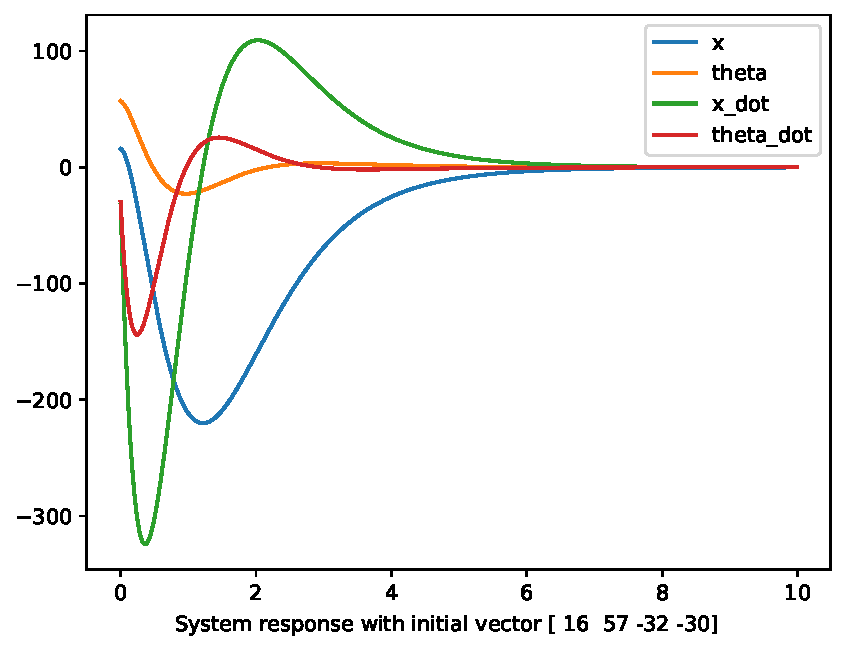
\includegraphics[width=0.49\linewidth]{../Task2/Fig1.pdf}
        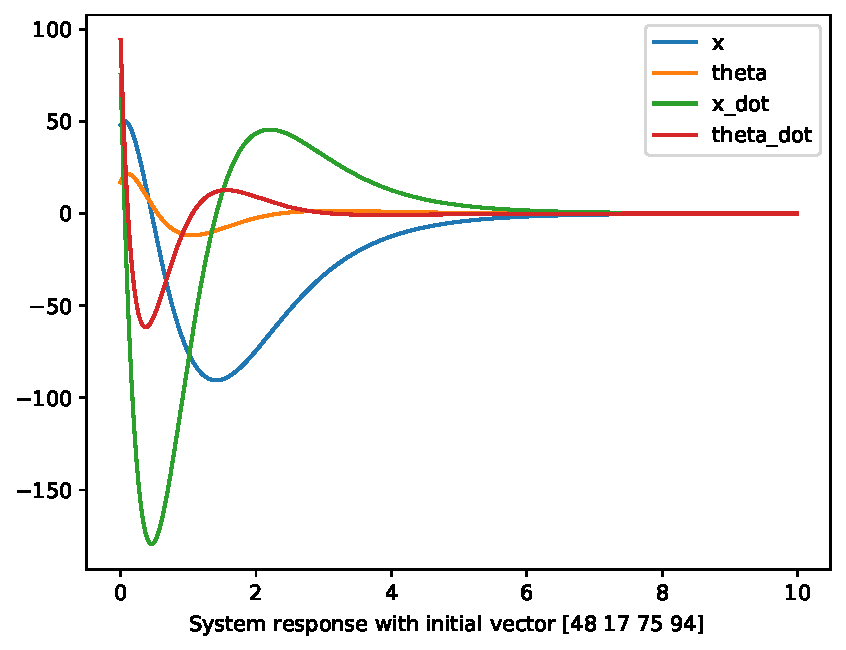
\includegraphics[width=0.49\linewidth]{../Task2/Fig2.pdf}
    \end{center}
    \begin{center}
        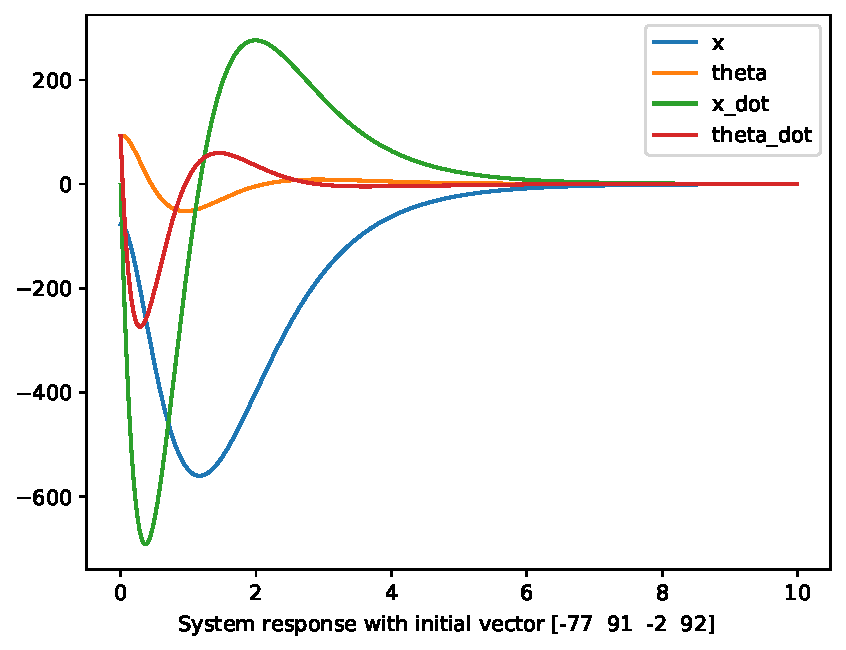
\includegraphics[width=0.49\linewidth]{../Task2/Fig3.pdf}
        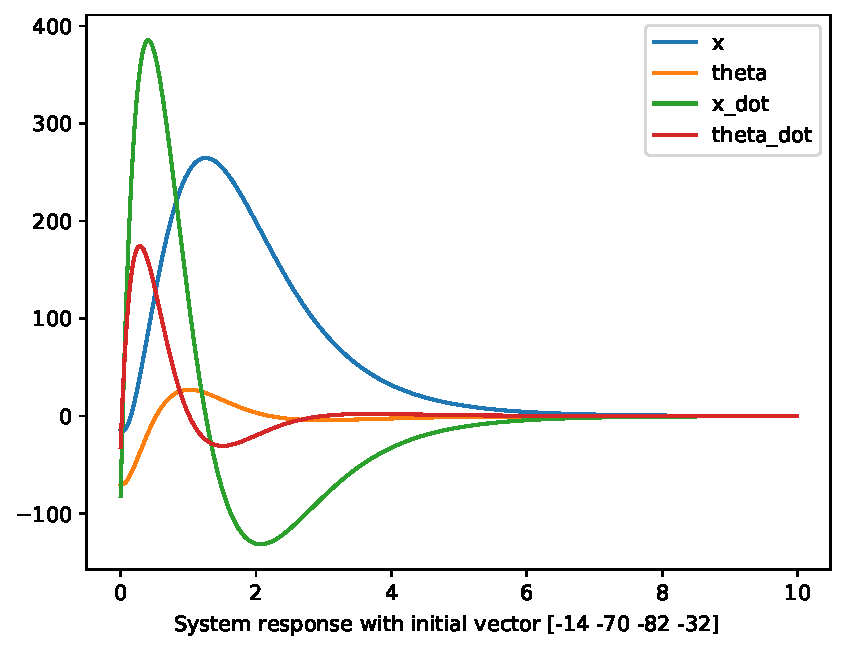
\includegraphics[width=0.49\linewidth]{../Task2/Fig4.pdf}
    \end{center}
    As it can be seen, all of them are going to stable state, with settling time
    about 5 seconds, but has large overshoot.\\
    The Python code of solution is located at \texttt{Task2/pole\_placement.py}.\\
    In Matlab I used \texttt{rlocus()} function to view Root-Locus plot of the 
    system. Unfortunately, \texttt{controlSystemDesigner} does not work properly
    on my version of Matlab, and shows wrong step response. So I looked at the 
    plot, and added and removed poles, controlling my step response.
    Initially, my Root-Locus plot was looking like this:\\
    \begin{center}
        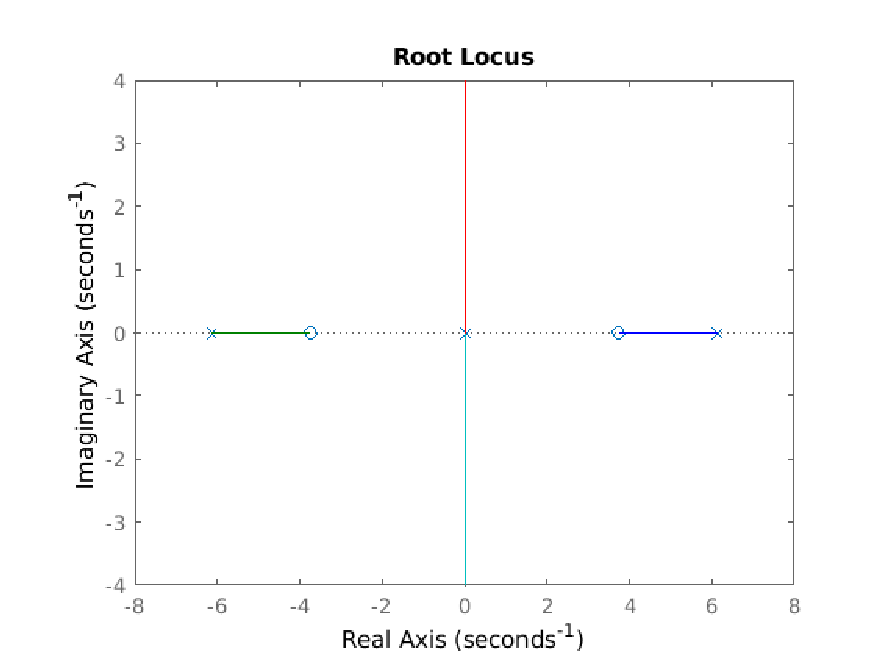
\includegraphics[width=0.7\linewidth]{../Task2/RLinit.pdf}
    \end{center}
    As it can be seen, there is positive pole, so i added zero at this point to 
    eliminate its influence. Then, I added two zeroes at the origin, and two poles
    at left half-plane, to make number of poles greater than number of zeroes, as 
    written \href{https://en.wikibooks.org/wiki/Control_Systems/Poles_and_Zeros}{there}.
    Now, my obtained Root-Locus plot is:
    \begin{center}
        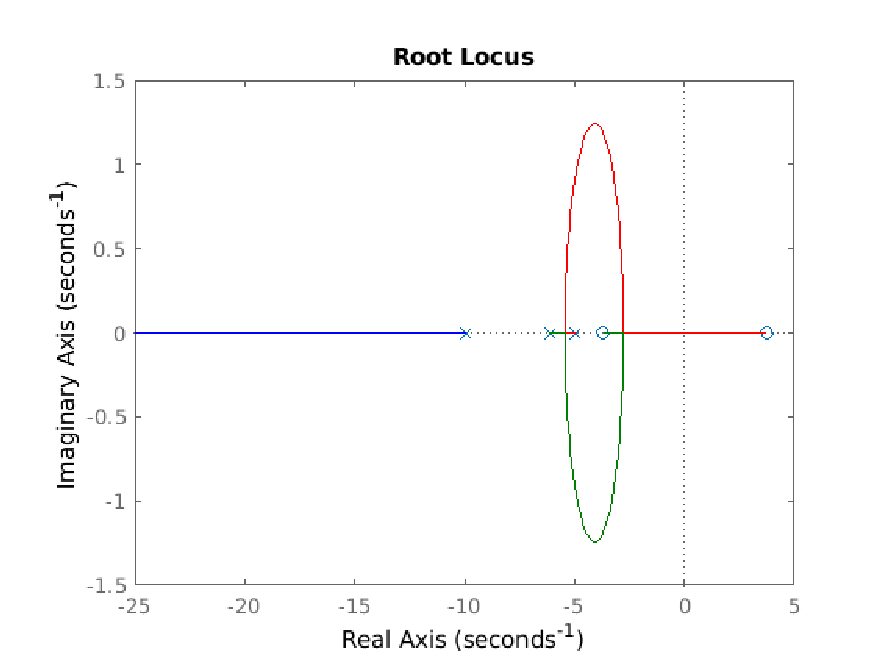
\includegraphics[width=0.7\linewidth]{../Task2/RLtuned.pdf}
    \end{center}
    And step response of the system, is here:
    \begin{center}
        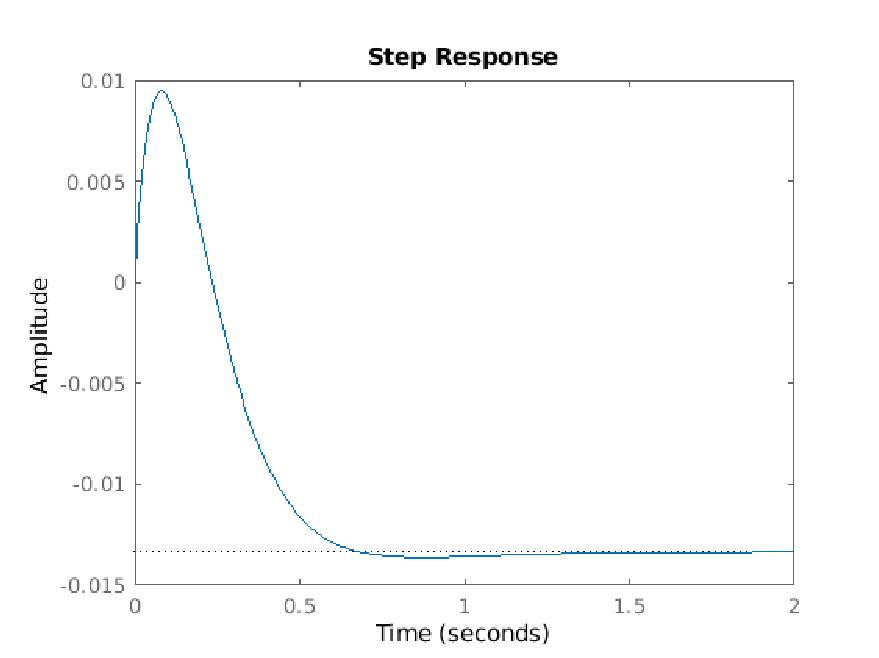
\includegraphics[width=0.7\linewidth]{../Task2/Step.pdf}
    \end{center}
    As it can be seen, output of the system is pretty stable, with steady-state 
    error around $2{e-2}$. Full code of the solution can be found in 
    \texttt{Task2/design.m}.
\section{Used software.}
\begin{itemize}
    \item Python 3.8.1
    \item Matlab R2018b 9.5.0
    \item draw.io
\end{itemize}
All software was run under Manjaro Linux with 5.4.18-rt kernel
\end{document}